\section{Results of the angular analysis}
 The angular analysis is performed using the same \qsq intervals as
 those used in the branching fraction measurement.  Results are
 reported for each \qsq interval in which the statistical significance
 of the signal is at least three standard deviations. This includes
 all of the \qsq intervals above the \jpsi resonance and the lowest
 \qsq bin.

\begin{table}[tbp]
\centering
\caption{Measured values of leptonic and hadronic angular observables,
  where the first uncertainties are statistical and the second
  systematic.}
\label{tab:afbresults}
\renewcommand{\arraystretch}{1.2}
\begin{tabular}{c|ccc}
 \qsq interval  [\gevgevcccc]   &            $A_{\rm FB}^\ell$      &       $f_{\rm L}$ 						&  $A_{\rm FB}^h$                    \\ \hline

0.1 -- 2.0   & $\phantom{-\,}0.37 \; ^{+\;0.37}_{-\;0.48} \,\pm\, 0.03$  	&   $0.56 \; ^{+\;0.23}_{-\;0.56}\,\pm\, 0.08$ 		& $-\;0.12 \; ^{+\;0.31}_{-\;0.28}\,\pm\, 0.15$	\\
11.0 -- 12.5 & $\phantom{-\,}0.01 \; ^{+\;0.19}_{-\;0.18} \,\pm\, 0.06$  	&   $0.40 \; ^{+\;0.37}_{-\;0.36}\,\pm\, 0.06$		& $-\;0.50 \; ^{+\;0.10}_{-\;0.00}\,\pm\, 0.04$	 \\
15.0 -- 16.0 & $-\,0.10 \; ^{+\;0.18}_{-\;0.16} \,\pm\, 0.03$  			&   $0.49 \; ^{+\;0.30}_{-\;0.30} \,\pm\, 0.05$ 	& $-\;0.19 \; ^{+\;0.14}_{-\;0.16}\,\pm\, 0.03$	\\	
16.0 -- 18.0 & $-\,0.07 \; ^{+\;0.13}_{-\;0.12} \,\pm\, 0.04$  			&   $0.68 \; ^{+\;0.15}_{-\;0.21} \,\pm\, 0.05$ 	& $-\;0.44 \; ^{+\;0.10}_{-\;0.05}\,\pm\, 0.03$	\\
18.0 -- 20.0 & $\phantom{-\,}0.01 \; ^{+\;0.15}_{-\;0.14} \,\pm\; 0.04$  	&   $0.62 \; ^{+\;0.24}_{-\;0.27}\,\pm\, 0.04$ 		& $-\;0.13 \; ^{+\;0.09}_{-\;0.12}\,\pm\, 0.03$	\\ \hline
15.0 -- 20.0 & $-\,0.05 \; ^{+\;0.09}_{-\;0.09} \,\pm\, 0.03$  			&   $0.61 \; ^{+\;0.11}_{-\;0.14} \,\pm\, 0.03$ 	& $-\;0.29 \; ^{+\;0.07}_{-\;0.07}\,\pm\, 0.03$	\\
\end{tabular}
\end{table}

\begin{figure}[ptb]
\centering
%%\includegraphics[width=0.49\textwidth]{images_and_tables/Angular/Afb_vs_q2_int_pred.pdf}
%%\includegraphics[width=0.49\textwidth]{images_and_tables/Angular/AfbB_vs_q2_int_pred.pdf}
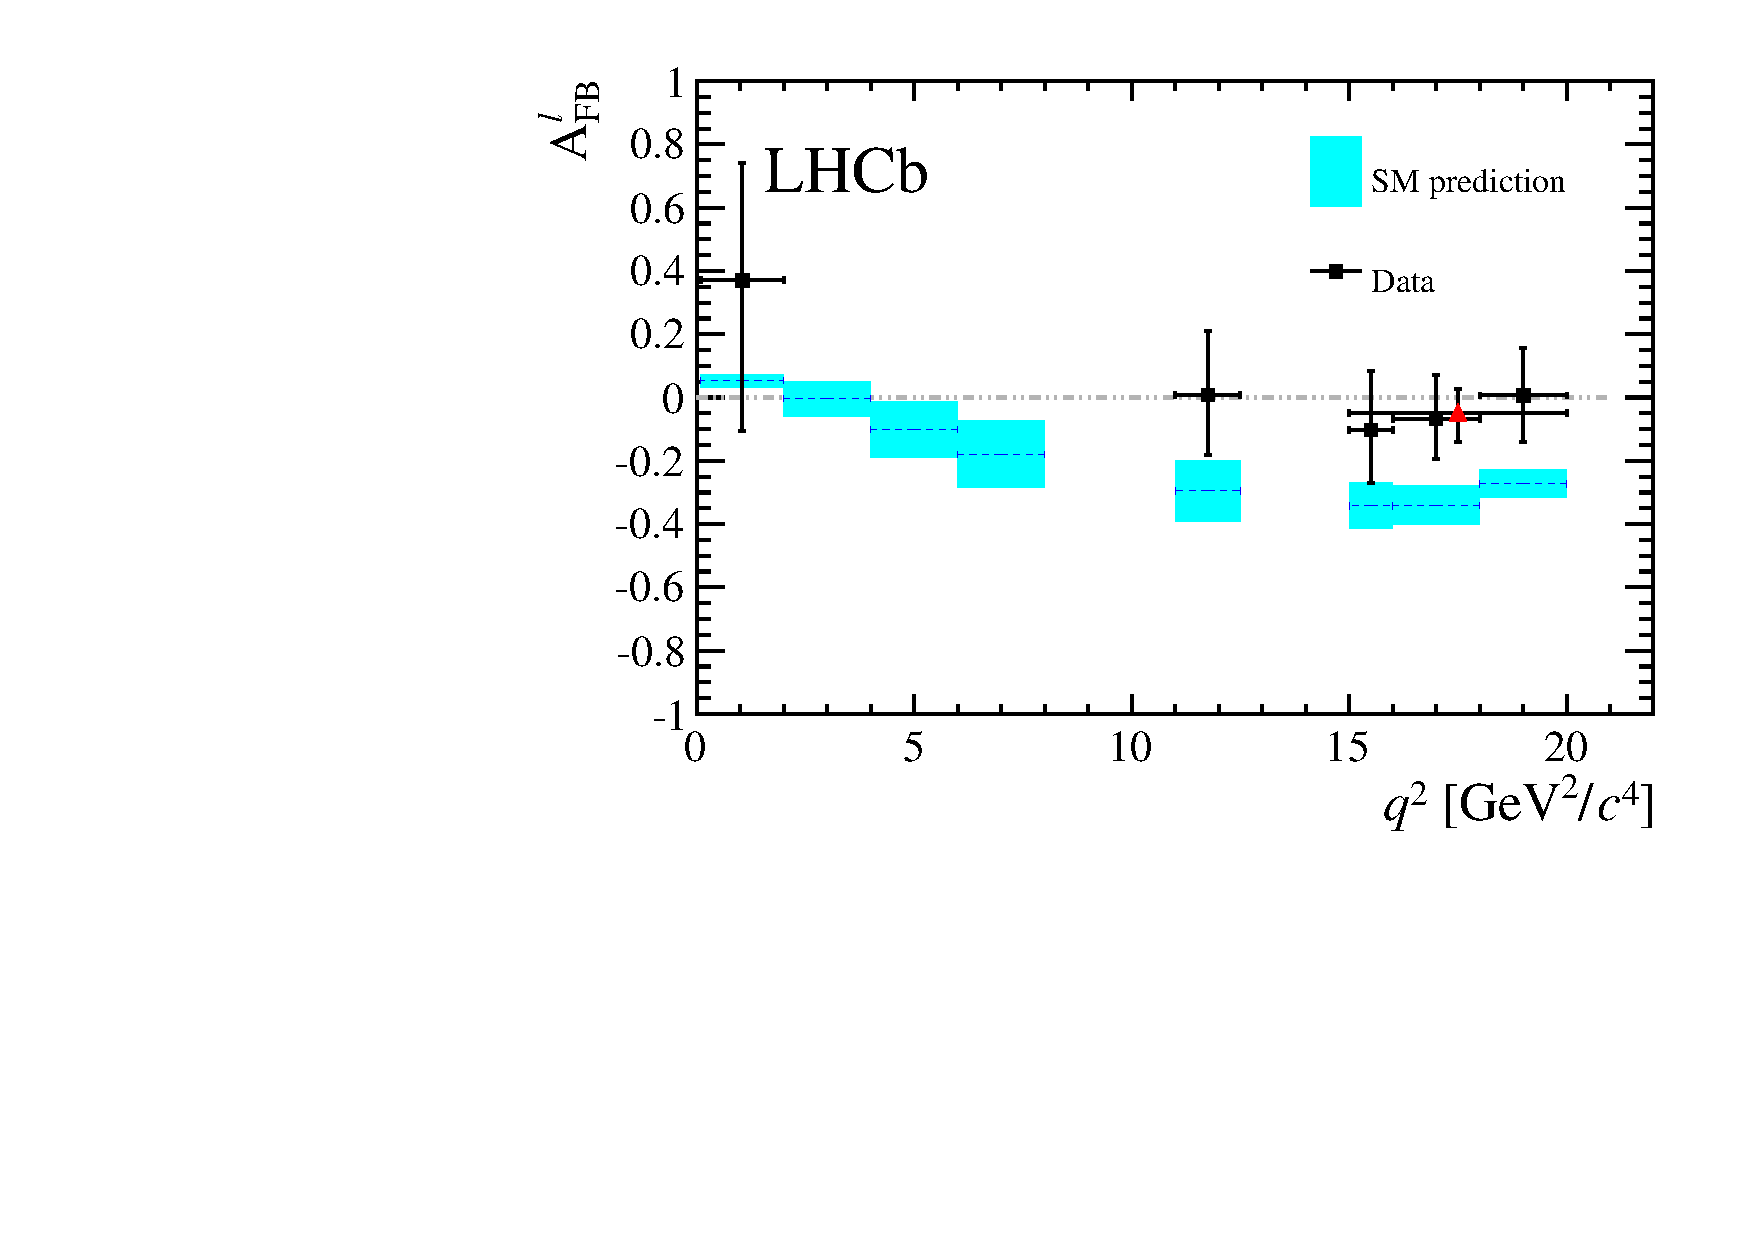
\includegraphics[width=0.49\textwidth]{figure8a.pdf}
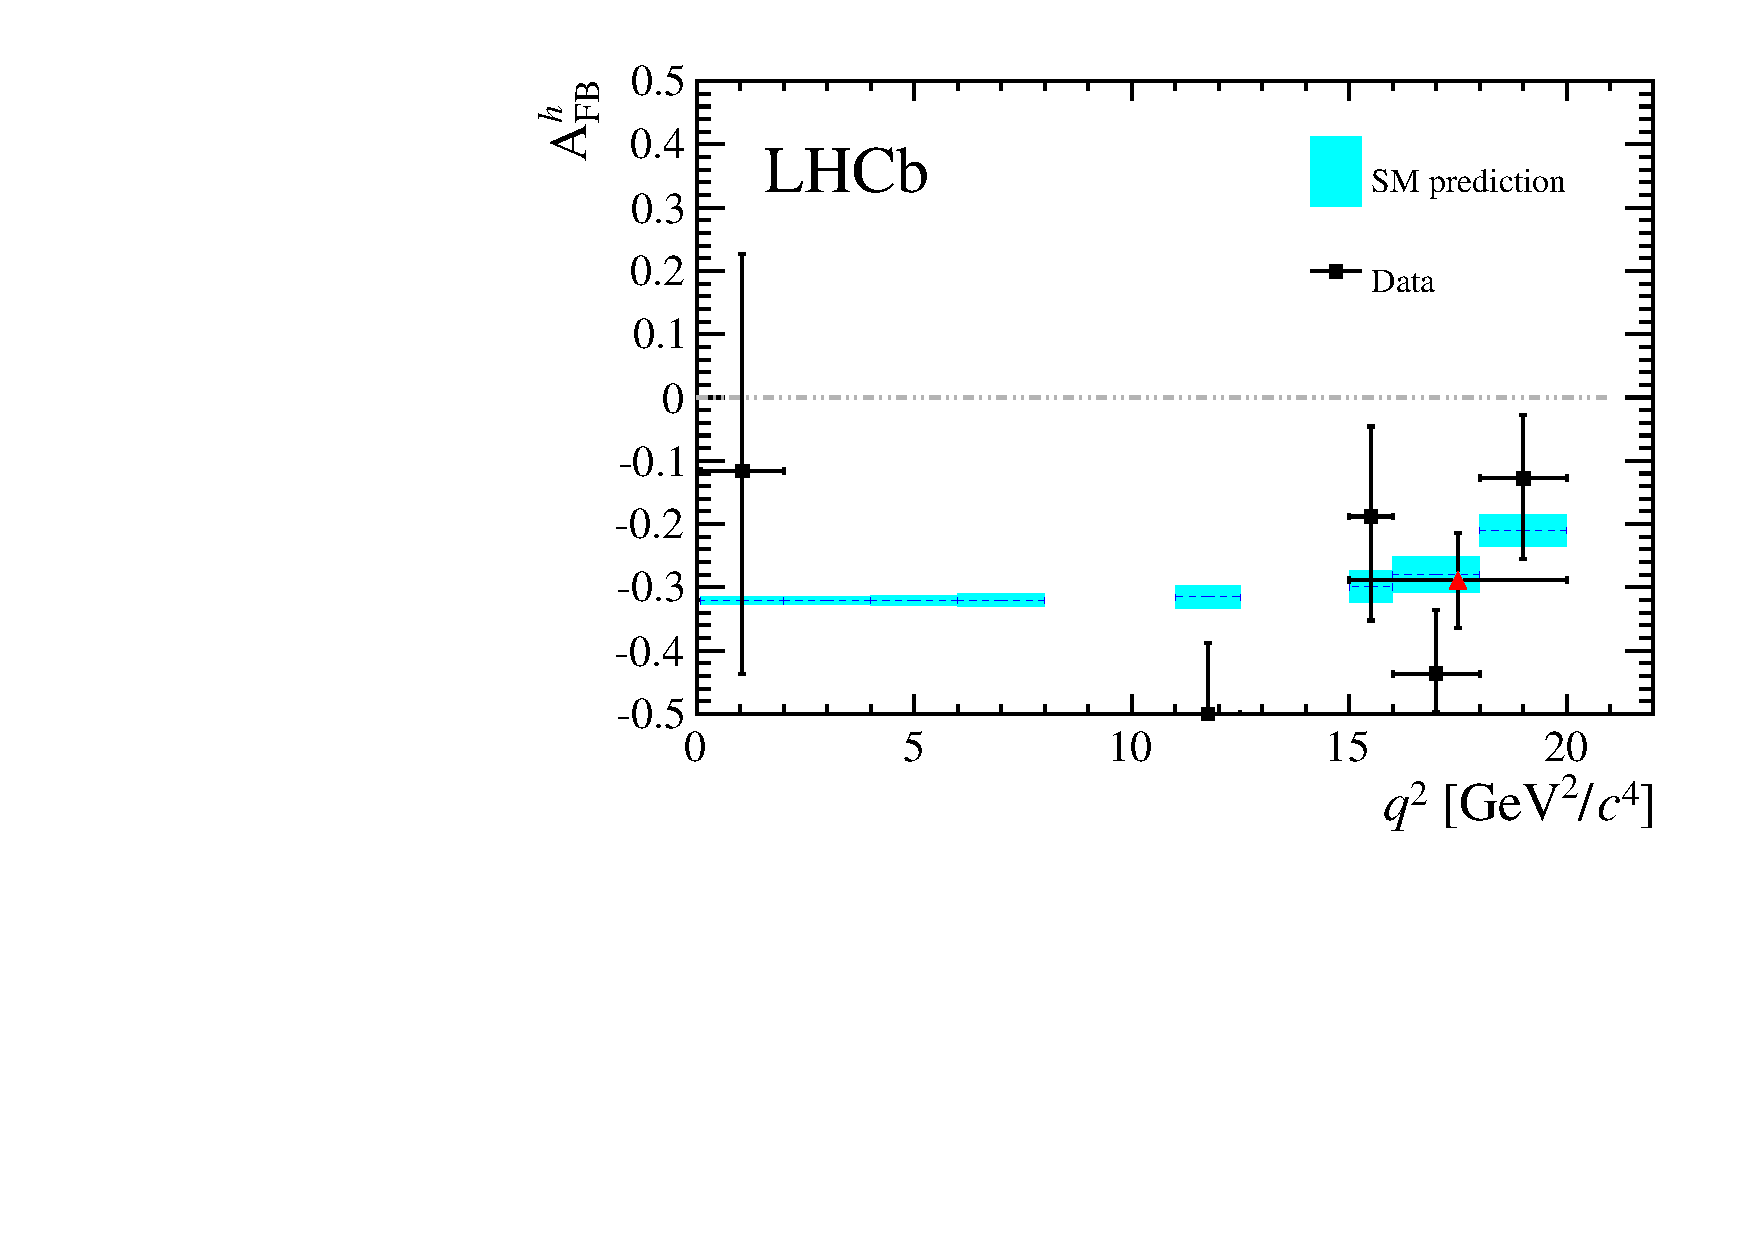
\includegraphics[width=0.49\textwidth]{figure8b.pdf}
\caption{Measured values of (left) the leptonic and (right) the hadronic
  forward-backward asymmetries in bins of \qsq.
  Data points are only shown for \qsq intervals where a statistically
  significant signal yield is found, see text for details.
  The (red) triangle represents the values for the $15 < \qsq < 20$ \gevgevcccc
  interval. Standard Model predictions are obtained from Ref.~\cite{Meinel:2014wua}.}
\label{fig:Afb_results}
\end{figure}

\begin{figure}[pbt]
\centering
%%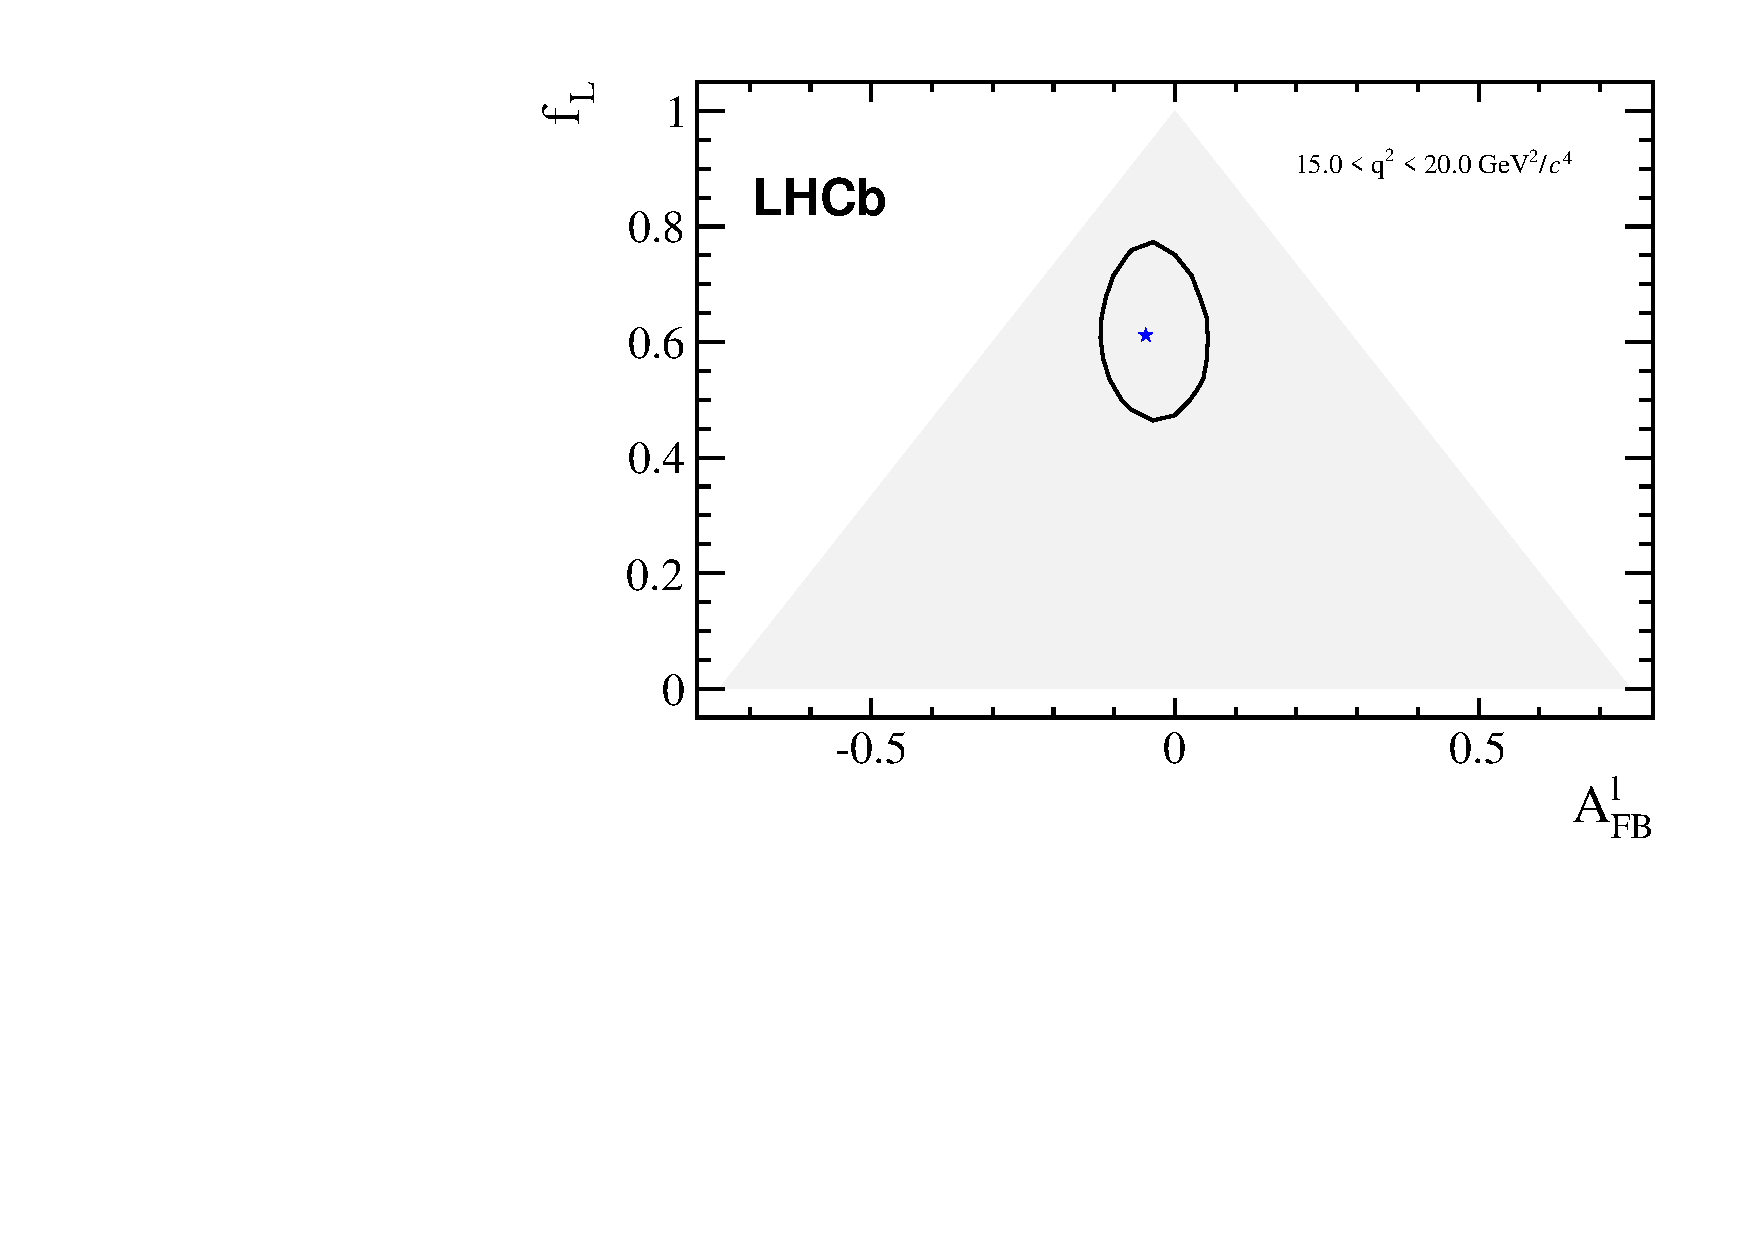
\includegraphics[width=0.8\textwidth]{images_and_tables/Angular/contours_1500_2000_1D.pdf}
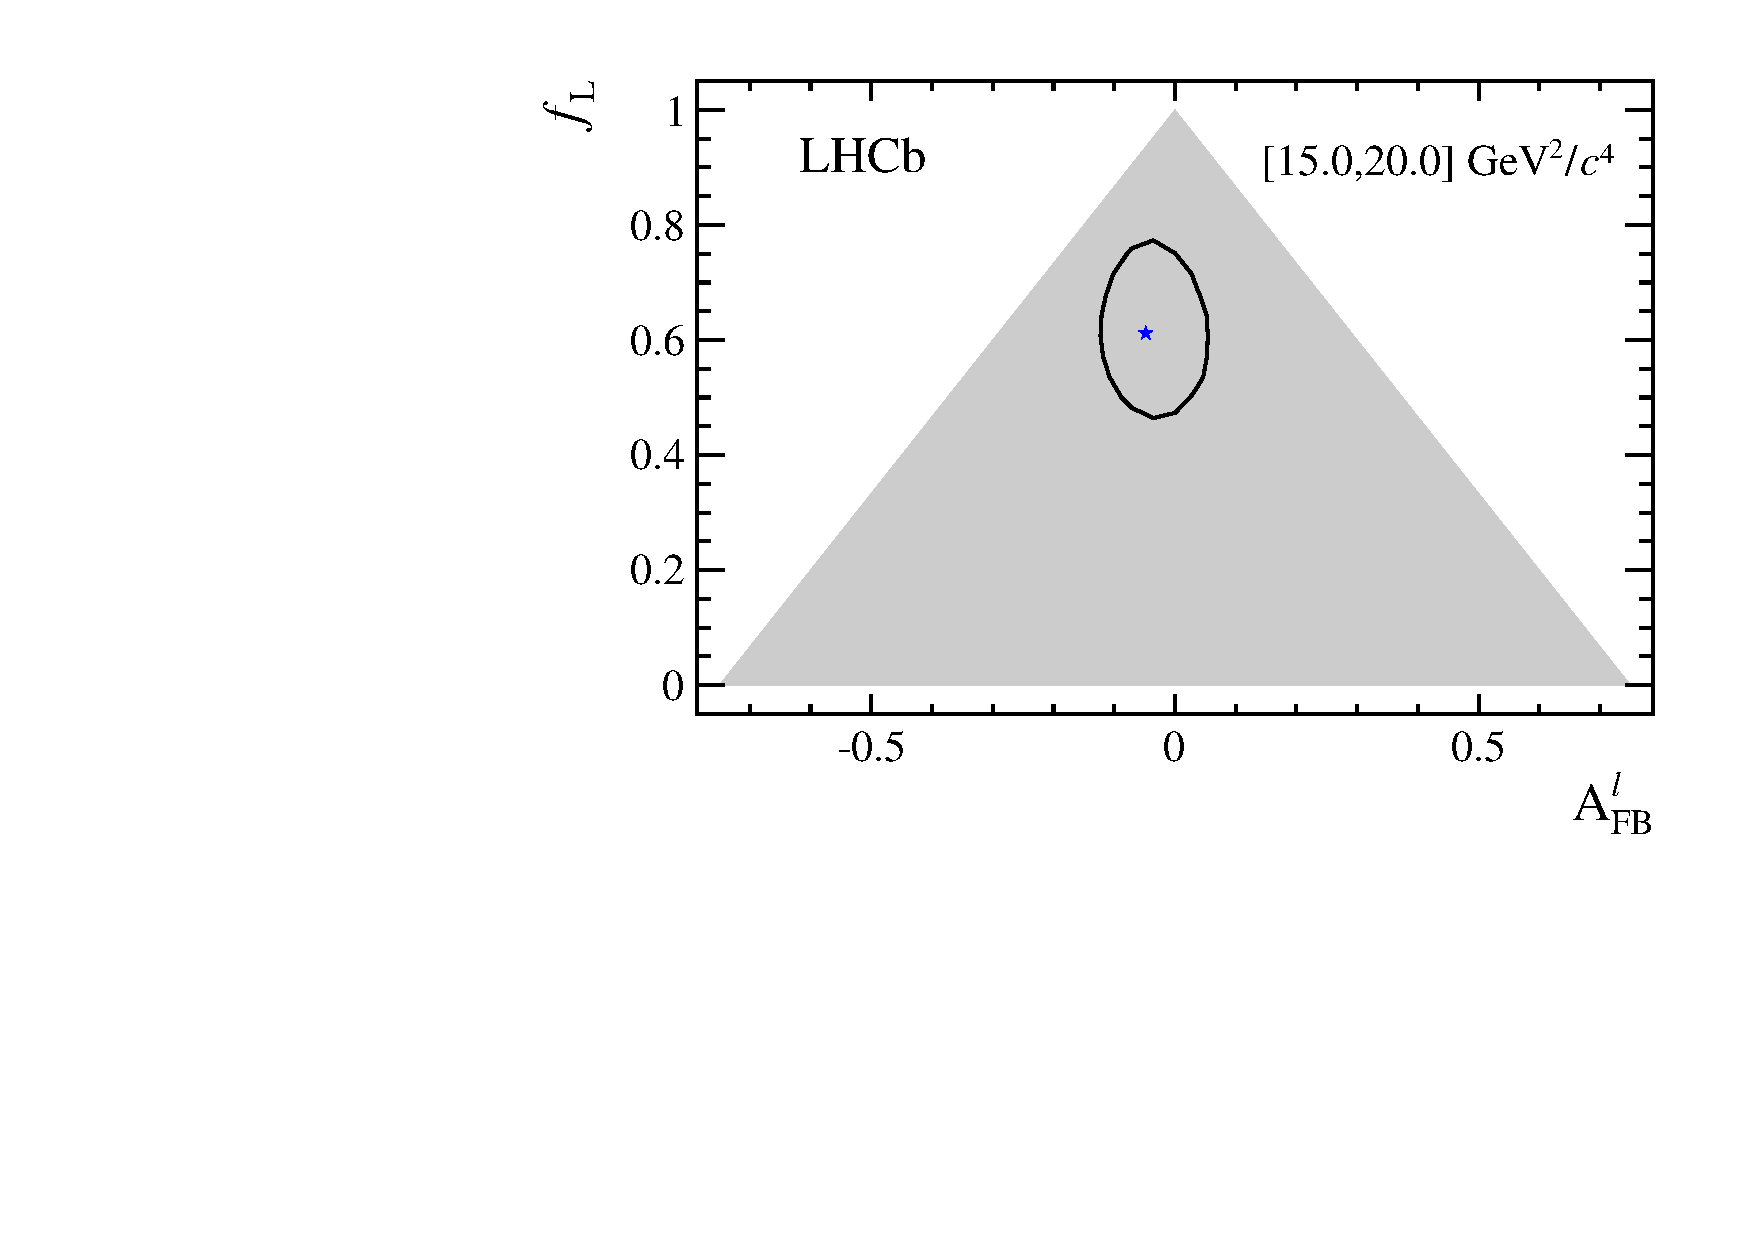
\includegraphics[width=0.8\textwidth]{figure9.pdf}
\caption{Two-dimensional 68\,\% CL region (black) as a
  function of $A_{\rm FB}^\ell$ and $f_{\rm L}$.  The shaded area
  represents the region where the PDF is positive over the complete $\cos
  \theta_{\ell}$ range. The best fit point is given by the (blue) star. }
\label{fig:contour_highq2}
\end{figure}

The measured values of the leptonic and hadronic forward-backward
asymmetries, $A_{\rm FB}^\ell$ and $A_{\rm FB}^h$, and the $f_{\rm L}$
observable are summarised in Table~\ref{tab:afbresults}, with the
asymmetries shown in Fig.~\ref{fig:Afb_results}. The statistical
uncertainties are obtained using the likelihood-ratio ordering
method\cite{Feldman:1997qc} where only one of the two observables at a
time is treated as the parameter of interest.  In this analysis
nuisance parameters were accounted for using the plug-in
method~\cite{woodroofe}.  In Fig.~\ref{fig:contour_highq2} the
statistical uncertainties on $A_{\rm FB}^\ell$ and $f_{\rm L}$ are
also reported (for the interval $15 < \qsq < 20$ \gevgevcccc) as a
two-dimensional 68\;\% confidence level (CL) region, where the
likelihood-ratio ordering method is applied by varying both
observables and therefore taking correlations into account.
Confidence regions for the other \qsq intervals are shown in
Fig.~\ref{fig:contours}, see Appendix.

